\documentclass[conference,a4paper]{IEEEtran}
\IEEEoverridecommandlockouts

\usepackage[a4paper,left=7.1mm,right=7.1mm,top=19.03mm,bottom=43mm]{geometry}
\usepackage{cite}
\usepackage{amsmath,amssymb,amsfonts}
\usepackage{graphicx}
\usepackage{booktabs}
\usepackage{textcomp}
\usepackage[T1]{fontenc}
\usepackage[hyphens]{url}
\usepackage[pdfborder={0 0 0}]{hyperref}

\graphicspath{{figures/}}

\begin{document}

\title{Subject-Independent Ictal versus Interictal Classification\\
from Single-Lead Wearable ECG on SeizeIT2}

\author{\IEEEauthorblockN{Poornima Madhu M}
\IEEEauthorblockA{\textit{Dept. of Electronics and Communication Engineering} \\
\textit{Amrita School of Engineering, Amrita Vishwa Vidyapeetham}\\
Coimbatore, India}}

\maketitle

\begin{abstract}
ECG studies often mix one patient's segments into both training and test
data, which can inflate scores. We compared ictal and interictal single-lead
ECG segments from 119 SeizeIT2 patients under subject-independent and
within-patient splits. Four classical classifiers used HRV, Poincar\'e and
morphology features; two 1D CNNs used raw windows. On 24 unseen patients a
random forest reached F1 0.895, against 0.373 for the best CNN. A
within-patient split raised it to 0.941. Ictal segments were shorter than
interictal ones, so this is state separability, not seizure prediction.
\end{abstract}

\begin{IEEEkeywords}
electrocardiography, epilepsy, heart rate variability, random forest,
SeizeIT2, subject-independent evaluation
\end{IEEEkeywords}

\section{Introduction}
Seizures are hard to anticipate, and scalp EEG is difficult to keep on for
long periods outside a hospital. A seizure also disturbs the autonomic
nervous system, so heart rate, heart-rate variability (HRV) and ECG
morphology change, and a single-lead ECG sensor is easier to wear than an
EEG cap \cite{Seifi2022,Abtahi2025}. The open SeizeIT2 dataset, released by
KU Leuven, offers such wearable recordings from 125 patients with focal
epilepsy: 11,640 hours in total, with 886 annotated seizures.

Clinicians describe a seizure in four phases: interictal (between seizures),
pre-ictal (before onset), ictal (the seizure itself) and post-ictal
(recovery). Detecting a seizure that is under way is a different problem
from predicting one that has not started. Prediction needs the pre-ictal
phase, whereas detection, and the classification task in this paper, only
needs to tell the ictal state from a quiet one. Cardiac changes can be
measured in all of these phases, which is why ECG is studied for both
problems. The question we ask is narrower: how well can ictal and interictal
ECG segments be told apart, and how much of that depends on the way the data
are split?

Many ECG studies report results from one random split. A recent analysis of
ECG-based prediction notes that variability between patients and within a
patient makes such results hard to compare \cite{Kalousios2025}. If segments
from one patient land in both the training and the test set, a classifier
can learn that patient's cardiac signature instead of anything
seizure-related. We could not find a direct measurement of this effect for
ECG on SeizeIT2.

We make three contributions.
\begin{itemize}
\item A pipeline that turns SeizeIT2 EDF recordings into labelled ictal and
interictal ECG segments and extracts HRV, Lorenz/Poincar\'e and morphology
features (Section~\ref{sec:methods}).
\item A side-by-side comparison of a subject-independent and a
within-patient split on the same feature table, with four classical
classifiers (Section~\ref{sec:results}).
\item A comparison with a one-dimensional CNN trained on raw ECG windows.
Under the same subject-independent split it scores far below the
feature-based random forest.
\end{itemize}
The task is to classify segments that are already known to be ictal or
interictal. It is not seizure prediction, and none of our numbers is a
warning time or a false-alarm rate. Section~\ref{sec:discussion} explains a
duration confound that limits what the scores can show.

\section{Literature Survey}\label{sec:lit}
\textbf{Classical machine learning on ECG features.} Seifi \textit{et al.}
trained SVM, $k$-NN and naive Bayes classifiers on 13 ECG features from 13
people in the Siena data and found naive Bayes the most suitable
\cite{Seifi2022}. Abtahi \textit{et al.} used heart-rate-variability (HRV),
Lorenz-plot and multifractal ECG features with a random forest and SHAP on
the EPILEPSIAE data, and reported 85.9\,\% accuracy and 84.6\,\% sensitivity
\cite{Abtahi2025}. Our feature families follow their work. Vishar
\textit{et al.} also applied a random forest, to pre-ictal stage prediction
\cite{Vishar2024}.

\textbf{Signal-processing and deep-feature approaches.} Perez-Sanchez
\textit{et al.} combined a maximal-overlap discrete wavelet packet transform
and a homogeneity index with a $k$-NN classifier on MIT-BIH data, reporting
93.25\,\% accuracy for a 20-min prediction interval \cite{PerezSanchez2024}.
Muralidharan \textit{et al.} used spectral whitening to remove normal
cardiac, respiratory and brain activity from the ECG before classification
\cite{Muralidharan2025}. Abarna \textit{et al.} used wavelet and variational
mode decomposition \cite{Abarna2023}. Muralidharan \textit{et al.} trained a
CNN with a joint cross-entropy and center loss on the TUSZ corpus, and
reported an AUROC of 0.8327 \cite{Muralidharan2023}. These figures are as
given in the cited papers and use different data and windows, so they cannot
be compared with each other or with our results.

\textbf{EEG--ECG and deep models.} Phomsiricharoenphant \textit{et al.}
studied EEG and ECG together with the Hilbert--Huang transform
\cite{Phomsiricharoenphant2014}. Subash \textit{et al.} proposed a framework
for early seizure detection \cite{Subash2024}, and Phuyal and Morshed used an
adversarial vision transformer with R\'enyi entropy on wearable EEG and ECG
\cite{Phuyal2026}. Truong \textit{et al.} showed that convolutional networks
can learn seizure-related patterns from intracranial and scalp EEG
\cite{Truong2018}. We test whether a comparable raw-signal network works on
single-lead ECG.

\textbf{Evaluation.} Kalousios \textit{et al.} trained patient-specific
models on 97 HRV features from 39 patients with 252 seizures. They reported a
mean ROC-AUC of 0.823 with non-causal evaluation and 0.569 with
pseudo-prospective evaluation, and pointed to variability between and within
patients \cite{Kalousios2025}. This gap between evaluation schemes is the
reason we compare split protocols.

\begin{figure}[t]
\centering
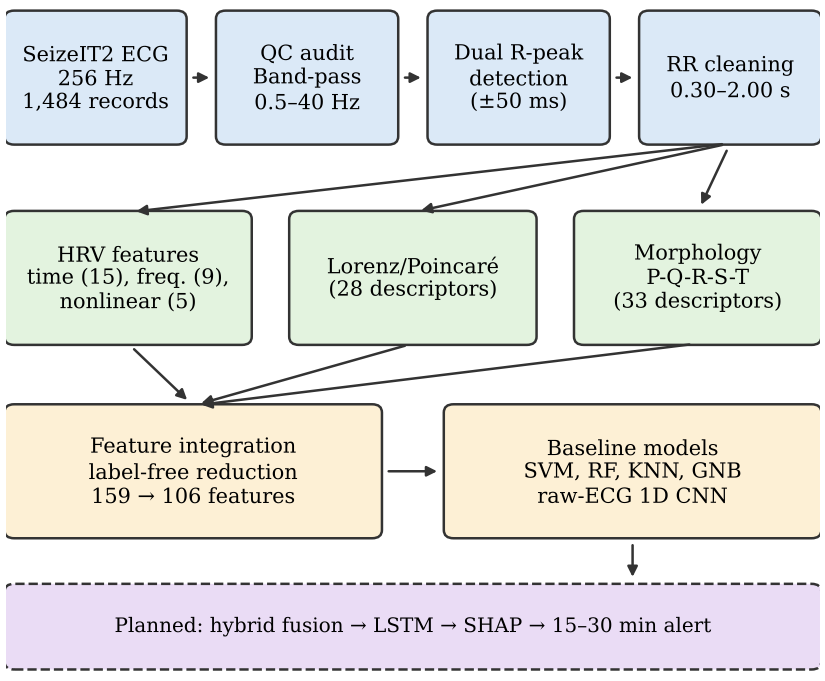
\includegraphics[width=0.92\columnwidth]{pipeline.png}
\caption{ECG processing pipeline. Solid boxes indicate implemented stages,
whereas the dashed box indicates the planned hybrid stage.}
\label{fig:pipeline}
\end{figure}

\begin{table}[t]
\caption{Segment dataset used in this study.}
\label{tab:dataset}
\centering
\footnotesize
\begin{tabular}{@{}lccc@{}}
\toprule
Class & Segments & Patients & Duration (s)\\
\midrule
Ictal & 851 & 119 & mean 58.6, median 33, range 2--962\\
Interictal & 822 & 119 & 300 (fixed)\\
Total & 1,673 & 119 & \\
\bottomrule
\end{tabular}
\end{table}

\begin{figure}[t]
\centering
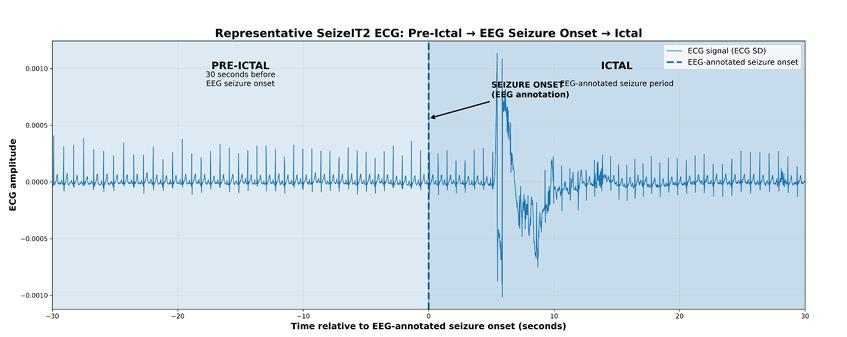
\includegraphics[width=\columnwidth]{ecg_onset.png}
\caption{Representative single-lead SeizeIT2 ECG 30\,s before and after an
EEG-annotated seizure onset (dashed line). The shaded part after onset is the
kind of signal an ictal segment contains; interictal segments in this study
lie at least 30\,min away from any seizure.}
\label{fig:ecg}
\end{figure}

\textbf{Research gap.} The studies above differ in data, window length and
validation. In the papers we reviewed we found none that measures how much a
patient-mixed split inflates ECG results on SeizeIT2. We measure that gap.

\section{Methods}\label{sec:methods}
Fig.~\ref{fig:pipeline} shows the pipeline. Everything was implemented in
Python.

\subsection{Data and Segment Extraction}
SeizeIT2 contains wearable recordings from 125 patients with focal epilepsy,
11,640\,h in total and 886 annotated seizures. The ECG is a single lead
sampled at 256\,Hz. Ictal segments were cut from the seizure onset and
duration given in each recording's events file (Fig.~\ref{fig:ecg}).
Interictal segments were fixed 5-min windows (300\,s) taken at least 30\,min
from every annotated seizure in the same recording. A run that has an events
file but no seizure annotation counts as seizure-free. This is an
operational definition, not a guarantee.

We ended up with 851 ictal and 822 interictal segments from 119 patients,
and every patient contributes both classes (Table~\ref{tab:dataset}). The
two classes differ sharply in length. Ictal segments have a mean duration of
58.6\,s and a median of 33\,s, with a range of 2--962\,s; 63.8\,\% of them
are shorter than 60\,s and only 14 reach 300\,s. This difference matters for
the features and for the interpretation of the results, and we come back to
it in Section~\ref{sec:discussion}.

\subsection{Preprocessing and Feature Extraction}
Each segment was filtered with a zero-phase fourth-order Butterworth
band-pass (0.5--40\,Hz). R-peaks were detected with the NeuroKit2 package,
and RR intervals outside 0.30--2.00\,s were discarded. Segments with fewer
than 10 clean RR intervals were flagged, and frequency-domain HRV was
computed only when at least 60 clean intervals spanning more than 60\,s were
available. Because many ictal segments are short, 411 segments were too
short for frequency-domain HRV and 106 had too few RR intervals. We left
those feature values missing instead of setting them to zero.

The feature table follows the usual HRV definitions and the feature families
used for seizure prediction in \cite{Abtahi2025}. It has five families:
time-domain HRV (e.g., MeanNN, SDNN, RMSSD, pNN50), frequency-domain HRV
(VLF, LF and HF power, LF/HF), nonlinear HRV (Poincar\'e SD1 and SD2, sample
entropy, DFA), Lorenz/Poincar\'e return-map descriptors, and beat-level
morphology descriptors (QRS width, amplitudes, QT approximation). We removed
segment length and count-type quality counters from the classifier inputs.
That left 95 candidate features.

Of the 95 candidates, 82 had at least 80\,\% non-missing values in both
classes of the training data, and the filter was computed on training data
only. The filter had a side effect that we want to state clearly. It removed
all 8 frequency-domain and all 5 nonlinear HRV features, because they were
missing for most ictal segments. Their training coverage was 0.97 in the
interictal class but only 0.35 for the frequency-domain features and
0.32--0.56 for the nonlinear ones in the ictal class. The classifiers
therefore see the 11 time-domain HRV, 27 Lorenz/Poincar\'e and 44 morphology
features only.

\subsection{Classical Classifiers}
We built four scikit-learn pipelines. All use median imputation, and all
except the random forest standardise the features: an RBF-kernel SVM
($C=1$, balanced class weights), a random forest (500 trees, minimum leaf
size 2, balanced subsample weights), $k$-nearest neighbours ($k=5$, distance
weighting) and Gaussian naive Bayes. We did not tune hyperparameters. The
settings are the ones in our scripts, so the scores should be read as a first
comparison and not as the best each model can do.

\subsection{Evaluation Metrics}
The ictal class is positive. With true and false positives and negatives
written TP, FP, TN and FN, we report precision, recall and $F_1$
\eqref{eq:prf} and the Matthews correlation coefficient (MCC) \eqref{eq:mcc}:
\begin{equation}
\text{Prec.}=\frac{TP}{TP+FP},\quad
\text{Rec.}=\frac{TP}{TP+FN},\quad
F_1=\frac{2\,\text{Prec.}\,\text{Rec.}}{\text{Prec.}+\text{Rec.}},
\label{eq:prf}
\end{equation}
\begin{equation}
\text{MCC}=\frac{TP\,TN-FP\,FN}{\sqrt{(TP+FP)(TP+FN)(TN+FP)(TN+FN)}}.
\label{eq:mcc}
\end{equation}
Balanced accuracy is the mean of recall and the recall of the interictal
class. ROC-AUC is the area under the curve of recall against the false
positive rate, and PR-AUC is the average precision. Accuracy alone would be
misleading for the CNN windows, where only 16.8\,\% are ictal, so we also
give recall, F1 and balanced accuracy.

\subsection{Raw-Signal CNN}
A one-dimensional CNN was trained on the extracted ECG without hand-crafted
features, using TensorFlow. Segments were cut into 10\,s windows with a 5\,s
stride at 256\,Hz. Each window was centred on its median, scaled by its
interquartile range and clipped to $\pm10$. The network has three
convolution layers (32, 64 and 128 filters with kernel sizes 7, 5 and 3),
batch normalisation and max pooling after the first two, global average
pooling, dropout of 0.35, a 64-unit dense layer, dropout of 0.25 and a
sigmoid output. We trained it with the Adam optimiser (learning rate
$10^{-3}$) and batch size 64. The baseline version used a 0.5 decision
threshold. The improved version added class weights, a validation set,
learning-rate reduction on plateau and a decision threshold chosen on the
validation set to maximise ictal F1.

\subsection{Experimental Setup}
\textbf{Protocols.} In the \textit{subject-independent} protocol, 20\,\% of
subjects were held out for testing (scikit-learn \texttt{GroupShuffleSplit},
seed 42, first split containing both classes), giving 95 training and 24
test subjects, and 1,491 training and 182 test segments. The test set holds
91 segments per class. No subject appears on both sides. All three
subject-wise experiments (classical models, baseline CNN, improved CNN) use
the same 24 test subjects, so their scores are comparable. For the CNN, the
test set expands to 6,315 windows, of which 1,064 are ictal and 5,251
interictal. The improved CNN further splits the 95 non-test subjects into 83
training and 12 validation subjects.

In the \textit{within-patient} protocol, segments of each patient and class
were split roughly 80:20 at random; a patient-class group with a single
segment stayed in training. This gives 1,302 training and 371 test segments,
with 93 patients present in both sets. We report it only to show how
optimistic such a split is. It is not a deployable setting.

\textbf{Metrics.} The ictal class is the positive class. We report accuracy,
balanced accuracy, precision, recall, F1, ROC-AUC and, for the classical
models, average precision (PR-AUC). Results come from a single split and a
single training run per model.

\textbf{Environment.} Code is Python with pandas, NumPy, SciPy, scikit-learn
and TensorFlow.

\begin{table*}[t]
\caption{Subject-independent test results (ictal class positive; 24 held-out subjects).}
\label{tab:classical}
\centering
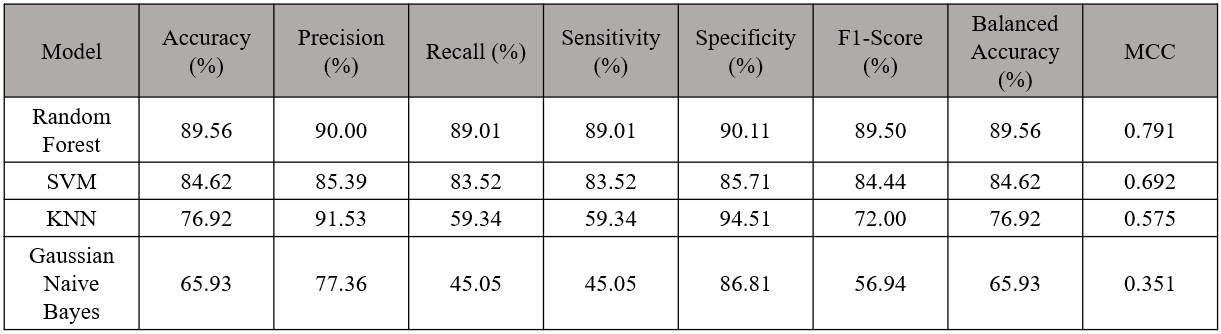
\includegraphics[width=0.82\textwidth]{classical_results.png}
\end{table*}

\begin{figure*}[t]
\centering
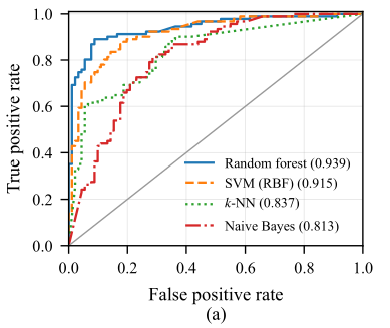
\includegraphics[width=0.337\textwidth]{roc_classical.pdf}\hspace{2em}%
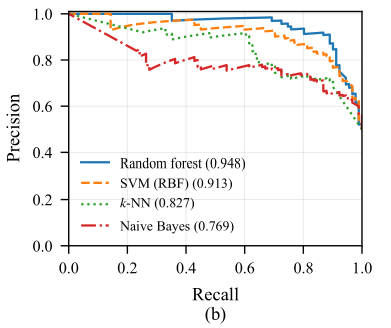
\includegraphics[width=0.337\textwidth]{pr_classical.pdf}
\caption{(a) ROC and (b) precision--recall curves of the four classical
models on the 24 held-out subjects. Area values are in parentheses.}
\label{fig:roc}
\end{figure*}

\begin{figure}[t]
\centering
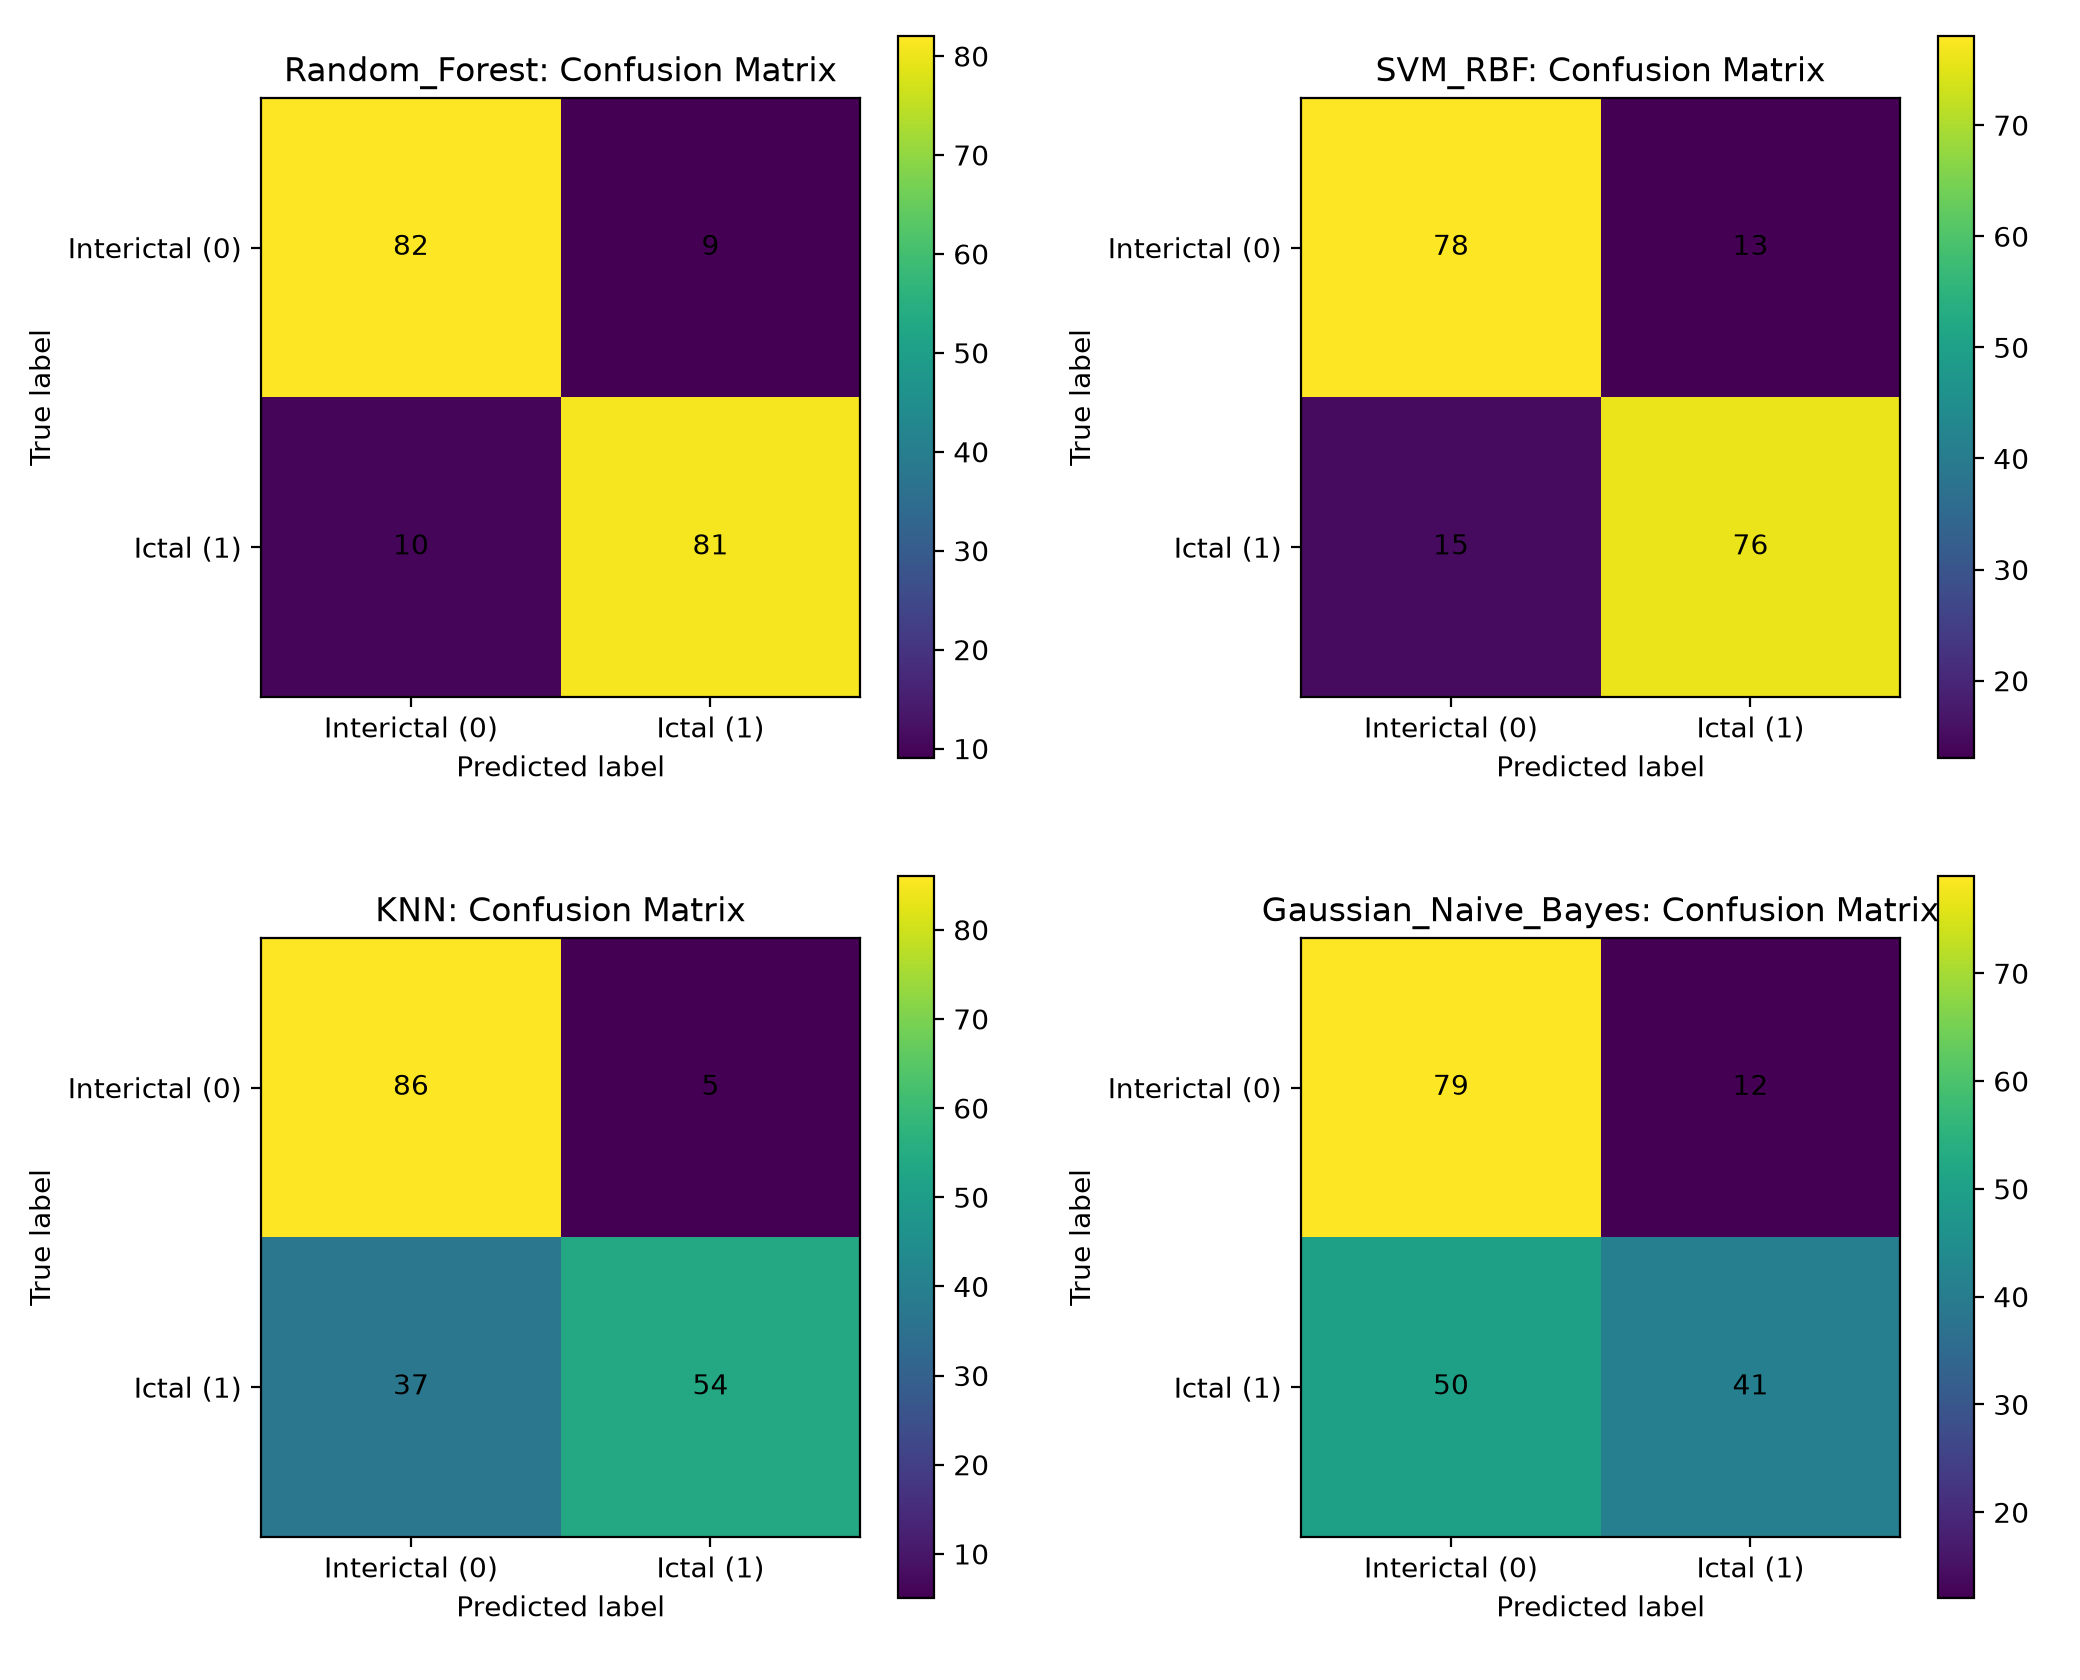
\includegraphics[width=\columnwidth]{confusion_classical.png}
\caption{Confusion matrices of the four classical models on the 182 test
segments of the 24 held-out subjects (subject-independent split).}
\label{fig:cm}
\end{figure}

\section{Results}\label{sec:results}
\subsection{Feature-Level Differences}\label{sec:featdiff}
Over all 1,673 segments, heart rate is clearly higher in ictal segments
(mean 92.3 against 75.3\,bpm), and MeanNN falls from 847.8 to 703.6\,ms
accordingly. This is the ictal tachycardia that often accompanies a seizure.
The variability measures overlap heavily: SDNN and RMSSD have large standard
deviations in both classes, and pNN50 is almost the same (27.5 against
28.9\,\%). Frequency-domain and entropy features are available for few ictal
segments (295 and 273 against 793 and 780), so their means come from
different subsets and should not be compared directly. These comparisons
are descriptive only; we ran no significance tests.

\subsection{Subject-Independent Classification}
Table~\ref{tab:classical} gives the results on the 24 held-out subjects. The
random forest has the best score on every metric except precision and
specificity, where $k$-NN is higher (0.915 and 0.945) at the cost of a
recall of 0.593. Fig.~\ref{fig:cm} shows the counts behind these numbers.
The forest makes 9 false alarms and 10 misses among 182 segments, and its
Matthews correlation coefficient is 0.791. Naive Bayes misses 50 of the 91
ictal segments. Fig.~\ref{fig:roc}(a,b) show the ROC and precision--recall
curves. The forest dominates the other three models over most of the range.

\subsection{Within-Patient versus Subject-Independent}
Repeating the experiment with the within-patient split, every model gains:
the F1 of the random forest rises from 0.895 to 0.941 and its ROC-AUC from
0.939 to 0.982, while the F1 of the SVM, $k$-NN and naive Bayes rises to
0.892, 0.838 and 0.606. The Matthews coefficient of the forest goes from
0.791 to 0.881, and its errors drop from 19 of 182 segments to 22 of 371.
The protocols also differ in test size (182 against 371 segments) and in
which segments are tested, so the gap is a rough indication and not a
controlled estimate. We have not yet repeated both protocols over many
random splits.

\subsection{Spread across Patients}
The pooled scores hide differences between patients. On the 24 test
patients, the random forest classified every segment correctly for 16
patients. The lowest per-patient accuracy was 0.50, three patients were
below 0.75, and the mean over patients was 0.92 (median 1.0). The test
patients contribute between 2 and 30 segments each, so a single wrong
segment moves the accuracy of a small patient a lot. The numbers show that
errors concentrate in a few patients, but they are too sparse to say why.

\subsection{Feature Importance}
Among the impurity importances of the random forest, the top feature is the
mean successive Lorenz difference (0.140), followed by the mean QRS-width
difference (0.068) and mean heart rate (0.044). Median heart rate and MeanNN
also appear in the top ten, as do several beat-to-beat difference measures
of QRS amplitude and R amplitude. The importance of heart rate agrees with
Section~\ref{sec:featdiff}. Impurity importance favours features with many
distinct values and can be shared among correlated features, so we read the
ranking as a rough guide and not as proof that a feature carries seizure
information.

\begin{figure}[t]
\centering
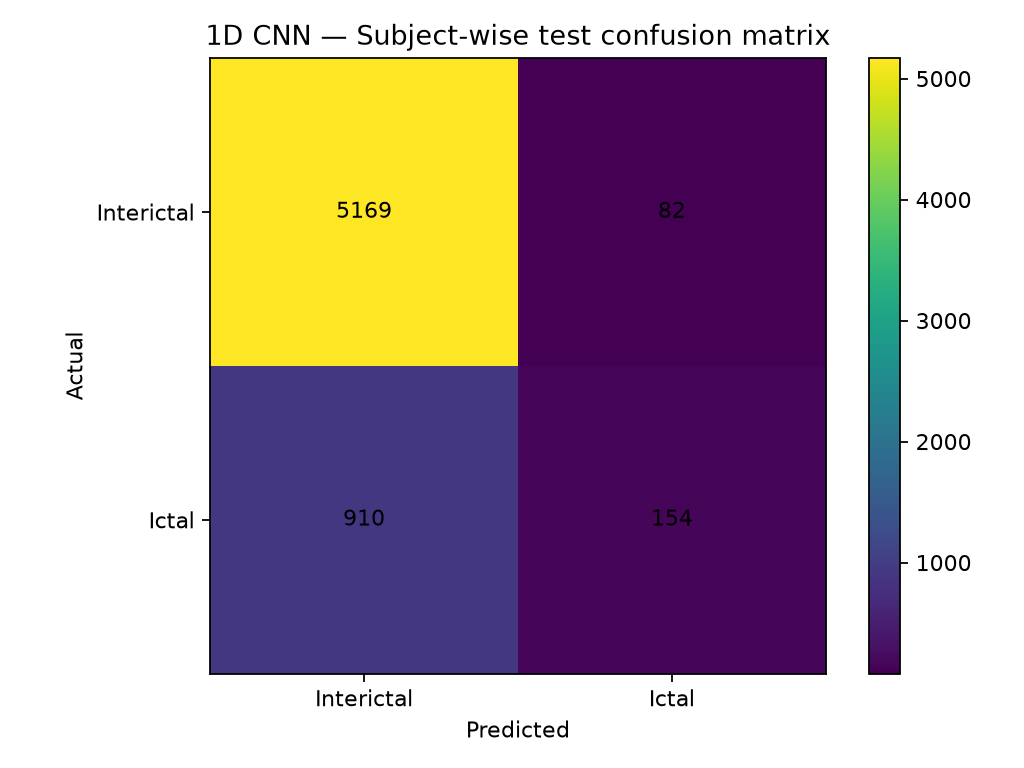
\includegraphics[width=0.8\columnwidth]{confusion_cnn.png}
\caption{Confusion matrix of the baseline 1D CNN on the 6,315 test windows of
the 24 held-out subjects.}
\label{fig:cnn}
\end{figure}

\subsection{Raw-Signal CNN}\label{sec:cnnres}
On the 6,315 test windows, 16.8\,\% of which are ictal, the baseline CNN
reached an accuracy of 0.843 and a balanced accuracy of 0.565, but its ictal
recall was only 0.145 (Fig.~\ref{fig:cnn}), and the accuracy is close to what
always predicting the interictal class would give. Class weights and a
validation-chosen threshold raised recall to 0.644 but cut precision from
0.653 to 0.263, which gives an F1 score of 0.373 (baseline 0.237) and a
balanced accuracy of 0.639. The CNN is scored on windows with a different
class balance, so these scores cannot be compared directly with the
segment-level Table~\ref{tab:classical}. Even so, the ROC-AUC gap (0.719 and
0.697 against 0.939) is large.

During training of the improved network, the training AUC rose to 0.919
after 15 epochs, while the validation AUC peaked at 0.743 and ended at
0.695. The best validation loss (0.486) came at epoch 9. The baseline
network stopped after 6 epochs. The widening gap between training and
validation curves means the network fits its training patients and does not
transfer to new ones.

\section{Discussion}\label{sec:discussion}
\subsection{What the Results Show}
The feature-based random forest separated the two states of unseen patients
far better than the raw-signal CNNs, and the within-patient split gave
higher scores for every classifier. Heart rate is the one feature with a
clear physiological reading here: it is higher in ictal segments, and it
ranks among the top features of the forest. Most of the other leading
features are beat-to-beat difference measures from the Lorenz plot and from
QRS and R amplitudes. We cannot say from our experiments whether they
reflect autonomic change during the seizure, movement artefact, or the
length of the segment.

\subsection{Relation to Earlier Work}
Our scores are not comparable with published ones. The studies in
Section~\ref{sec:lit} use other datasets, other segment definitions and, in
several cases, a pre-ictal target. The one comparison we can draw is about
the evaluation scheme. Kalousios \textit{et al.} found a mean ROC-AUC of
0.823 with non-causal evaluation but 0.569 with pseudo-prospective
evaluation \cite{Kalousios2025}. We saw the same direction on a different
task: scores fall when the test condition gets closer to real use. In our
case the step is from a within-patient to a subject-independent split, and
the random-forest ROC-AUC falls from 0.982 to 0.939. The drop is smaller
than theirs, but our task is also easier, because the classes are ictal
against distant interictal segments and not pre-ictal against interictal
ones.

\subsection{Why the CNN Fell Behind}
We did not run ablations, so the following are hypotheses. First, the window
normalisation removes absolute amplitude, which is one of the morphology
cues the forest can use. Second, a 10\,s window holds only a handful of
beats, so a network on a single window cannot see the longer-range rhythm
that features computed over a whole segment capture. Third, 119 patients may
simply be too few for a network to learn a patient-independent
representation from raw ECG, which fits the training--validation gap in
Section~\ref{sec:cnnres}. We also did not tune the CNN, and the two networks
are a small sample of possible designs.

\subsection{Limitations}
\textbf{Duration confound.} Interictal segments are all 300\,s long while
ictal segments average 58.6\,s, and 63.8\,\% of them are shorter than 60\,s.
We excluded length and count features, but many HRV statistics depend on the
number of beats. The missing-value pattern is also informative: the filter
removed the frequency-domain and nonlinear HRV features because they are
missing for most ictal segments, and the median imputation we used for the
remaining gaps could still let a classifier tell short from long. The random
forest may therefore partly separate short from long segments. We have not
yet rerun the experiment with interictal windows cut to the ictal length
distribution, and until then the headline scores cannot be read as a measure
of seizure-specific information.

\textbf{Not prediction.} The task separates segments that are known to be
ictal from those at least 30\,min away from a seizure. It does not test
whether a pre-ictal state can be recognised in time, and no warning horizon
or false-alarm rate is measured. Many studies in Section~\ref{sec:lit}
address that harder problem, so their results do not compare with ours.

\textbf{Evidence.} Results come from one split and one run, without
confidence intervals, and the test set has only 182 segments from 24
patients. The interictal label relies on the dataset annotations alone. The
feature-based and CNN comparison also differs in unit of analysis and input
length. We tuned no hyperparameters, and we made no comparison with
published methods on identical data, because no such numbers exist for this
segment definition. Finally, there is no trivial baseline such as a
heart-rate threshold. Given Section~\ref{sec:featdiff}, a simple heart-rate
rule might score well, and a reviewer would reasonably ask for it.

\subsection{Reproducibility and Data}
SeizeIT2 is an open dataset. Our extraction, feature and model scripts, the
per-segment predictions and the split membership lists are saved with the
project, which allows the tables and figures above to be regenerated.
Hardware and library versions are not reported in this paper.

\section{Conclusion}
On single-lead SeizeIT2 ECG, a random forest on 82 features separated ictal
from interictal segments of 24 unseen patients with an F1 score of 0.895 and
a ROC-AUC of 0.939, while raw-signal CNNs reached an F1 score of at most
0.373 under the same split. A within-patient split gave higher scores for
every classifier, so patient-mixed splits overstate what a deployed system
would achieve. Heart rate was higher in ictal segments and was among the
most important features.

Three things limit these conclusions: the duration difference between the
classes, the single split and the absence of any prediction horizon. Our
next steps follow from them. We will rerun the comparison with
length-matched interictal windows and with repeated splits and confidence
intervals, and add a heart-rate-only baseline. After that we plan to move to
pre-ictal windows with a 15--30\,min horizon and to report the seizure
prediction horizon and the false-positive rate per hour. This planned work
has not been done, and nothing in this paper should be read as a prediction
result.

\newcommand{\doi}[1]{doi: \href{https://doi.org/#1}{#1}}

\begin{thebibliography}{00}
\bibitem{Seifi2022} B. Seifi, M. Barfi, and M. Esmaeilpour, ``ECG-based
prediction of epileptic seizures using machine learning methods,'' in
\textit{Proc. 9th Iran. Joint Congr. Fuzzy Intell. Syst. (CFIS)}, 2022,
pp.~1--7, \doi{10.1109/CFIS54774.2022.9756421}.

\bibitem{Abtahi2025} A. Abtahi, P. Ryvlin, and A. Aminifar,
``Identification of relevant ECG features for epileptic seizure prediction
using interpretable machine learning,'' \textit{IEEE Access}, vol.~13,
pp.~111\,293--111\,303, 2025, \doi{10.1109/ACCESS.2025.3583461}.

\bibitem{Kalousios2025} S. Kalousios \textit{et al.}, ``ECG-based epileptic
seizure prediction: Challenges of current data-driven models,''
\textit{Epilepsia Open}, vol.~10, no.~1, pp.~143--154, 2025,
\doi{10.1002/epi4.13073}.

\bibitem{Vishar2024} M. A. M. Vishar, D. Hepsiba, R. Prasanna, and L. D. V.
Anand, ``Machine learning-based early seizure detection: A random forest
classifier approach for pre-ictal stage prediction in epilepsy,'' in
\textit{Proc. 10th Int. Conf. Bio Signals, Images, Instrum. (ICBSII)}, 2024,
\doi{10.1109/ICBSII61384.2024.10564015}.

\bibitem{PerezSanchez2024} A. V. Perez-Sanchez, J. P. Amezquita-Sanchez, M.
Valtierra-Rodriguez, and H. Adeli, ``A new epileptic seizure prediction model
based on maximal overlap discrete wavelet packet transform, homogeneity
index, and machine learning using ECG signals,'' \textit{Biomed. Signal
Process. Control}, vol.~88, p.~105659, 2024,
\doi{10.1016/j.bspc.2023.105659}.

\bibitem{Muralidharan2025} P. Muralidharan, C. S. Kumar, R. Sankaran, and
K. I. Ramachandran, ``Seizure information enrichment in ECG through spectral
whitening for improving epileptic seizure prediction,'' \textit{Comput.
Biol. Med.}, vol.~189, p.~109929, 2025,
\doi{10.1016/j.compbiomed.2025.109929}.

\bibitem{Abarna2023} B. Abarna, C. S. Kumar, P. Muralidharan, S. Gopinath,
and A. A. Kumar, ``Improving the performance of ECG-based epileptic seizure
prediction using wavelet and variational mode decomposition,'' in
\textit{Proc. 4th IEEE Annu. Flagship India Council Int. Subsections Conf.
(INDISCON)}, 2023, pp.~1--7, \doi{10.1109/INDISCON58499.2023.10270397}.

\bibitem{Muralidharan2023} P. Muralidharan \textit{et al.}, ``Improving the
performance of epileptic seizure prediction using supervised clustering of
deep features,'' in \textit{Proc. 14th Int. Conf. Comput. Commun. Netw.
Technol. (ICCCNT)}, 2023, pp.~1--7,
\doi{10.1109/ICCCNT56998.2023.10307308}.

\bibitem{Phomsiricharoenphant2014} W. Phomsiricharoenphant, S.
Ongwattanakul, and Y. Wongsawat, ``The preliminary study of EEG and ECG for
epileptic seizure prediction based on Hilbert-Huang transform,'' in
\textit{Proc. 7th Biomed. Eng. Int. Conf. (BMEiCON)}, 2014,
\doi{10.1109/BMEiCON.2014.7017433}.

\bibitem{Subash2024} K. Subash, A. Saravanan, and B. Padmavathi, ``A
framework for suggesting a new methodology for early detection of epilepsy
seizure,'' in \textit{Proc. Int. Conf. Inventive Comput. Technol. (ICICT)},
2024, \doi{10.1109/ICICT60155.2024.10544956}.

\bibitem{Phuyal2026} A. K. Phuyal and B. I. Morshed, ``AdViT-RE:
Adversarial vision transformer with R\'enyi entropy for multimodal epileptic
seizure prediction using wearable EEG and ECG,'' in \textit{Proc. IEEE Int.
Conf. Electro Inf. Technol. (eIT)}, 2026,
\doi{10.1109/eIT68936.2026.11670343}.

\bibitem{Truong2018} N. D. Truong \textit{et al.}, ``Convolutional neural
networks for seizure prediction using intracranial and scalp
electroencephalogram,'' \textit{Neural Netw.}, vol.~105, pp.~104--111, 2018,
\doi{10.1016/j.neunet.2018.04.018}.
\end{thebibliography}

\end{document}
